\subsection{Controlador}
El controlador en un MVC es el responsable de recibir y procesar la entrada del usuario y actualizar el modelo. En esta práctica, dicha responsabilidad es la de generar un conjunto de puntos de una distribución en concreto, la de encontrar \textit{n} parejas que maximicen o minimicen su distancia y generar estadísticas basadas en los datos del modelo.

\subsubsection{Diseño}
El controlador se separa en tres grandes secciones como ya se ha mencionado previamente. \\

Para la generación de datos, se definen un conjunto de funciones que, mediante el objeto interno que permite generar datos aleatorios, retorna el siguiente valor de la distribución que caiga dentro de unas \say{boundaries} específicas. De esta manera, nos aseguramos que todos los datos son fácilmente visibles a la hora de visualizaros; Facilitando así las futuras visualizaciones de las soluciones. Actualmente, el software permite la visualización de la distribución Uniforme, Gausiana, Exponencial desplazada y Bernoulli. Adicionalmente, esta generación de datos utiliza una semilla, por lo que el usuario fácilmente puede replicar resultados. \\

Para la generación de estadísticas, se recogen los datos del modelo y se efectúan medias, máximos y mínimos para visualizarlos claramente en la ventada de estadísticas (\ref{fig:Ejemplo stats Algt}). De esta manera, ofrecemos al usuario un feedback sobre la ejecución del algoritmo que puede ser usada para contrastar los resultados en un estudio formal.\\

Finalmente, el cálculo de distancias mínimas y máximas se efectúan bajo los datos presentes en el modelo aplicando el respectivo algoritmo dependiendo de la petición obtenida del Hub. A continuación se entrará en más detalle la implementación de los algoritmos y su proceso de diseño.

\subsubsection{Algoritmos}
Para esta práctica, se han implementado la búsqueda de distancias mínimas y máximas con un coste asintótico $O(n^2)$ y la búsqueda de distancias mínimas en $O(nlogn)$.\\

Para las implementaciones $O(n^2)$, los algoritmos iteran por todos puntos de datos y calculan todas las posibles permutaciones entre ellos, guardando dinámicamente las mejores soluciones en el respectivo \say{array}. Asintóticamente hablando, debido a que el software está generalizado para \textit{m} soluciones, presenta un coste de $O(n^2 · mlogm)$ ya que se efectúa una ordenación de los datos para asegurar que siempre se guardan las mejores soluciones. Adicionalmente, debido a que se ha considerado que el número de soluciones a encontrar no sería especialmente grande, se ha decidido no optimizar el algoritmo a $O(n^2 m)$ para mantener una mejor legibilidad y calidad del código, ya que se podría implementar una modificación del las actuales soluciones en coste lineal  y guardar localmente la mejor/peor solución para poder compararlo con la solución actual.\\

Para la implementación $O(nlogn)$ de las distancias mínimas, como el título del documento indica, se ha decidido usar \say{Divide \& Conquer} para ir dividiendo el espacio de puntos logarítmicamente. Este se divide en dos partes, un inicial estado donde se preparan los datos y una segunda, y más computacionalmente pesada, donde se computan todas las distancias. Inicialmente, se recogen los datos del modelo y se ordenan por su componente \textit{x}, de esta manera facilitamos la separación de los datos en los diferentes sectores en el siguiente apartado. El segundo apartado es un algoritmo recursivo cuyos parámetros permiten identificar el \say{slice} de datos que se está tratando actualmente y los datos a tomar. La condición de salida de este algoritmo se cumple cuando el \say{slice} de datos solo presenta dos puntos. En tal caso, se genera un \say{array} de soluciones de \textit{m} posiciones donde en la primera posición se encuentra la única solución y las restantes presentan distancias imposibles. En este caso, debido a que se están trabajando con \say{arrays}, el tiempo de composición de las soluciones es de $O(nlogn)$ al tener que obtener ambas soluciones, ordenarlas y producir un \say{slice} con las menores distancias. Finalmente, se debe revisar los puntos intermedios entre los dos sectores, ya que podrían existir mejores soluciones. Para ello, se toma la menor distancia y se crea un \say{slice} de datos desde el punto intermedio con $2*menor\_distancia$ como el diámetro. De esta manera, aseguramos que solo se tomen aquellos puntos que puedan ofrecer una mejor solución. Finalmente, se generan todas las posibles permutaciones entre ellos mediante un algoritmo $O(n^2)$ similar al expuesto previamente. Como se acaba de comentar, uno podría pensar que, debido a que por cada ejecución del algoritmo recursivo se efectúa un \say{snippet} de código con complejidad asintótica $O(n^2)$ el algoritmo presentaría dicha complejidad. Esto es cierto en distribuciones cuya densidad de puntos en los valores centrales es significativamente mayor, como podría ser la Gausiana. Sin embargo, para distribuciones equiprobables, como la Uniforme, sabemos que la cantidad de puntos de cada conjunto que están dentro de un sector tiende a la raíz cuadrada de los puntos en total. Debido a esto, se podría considerar que este algoritmo es $O(nlogn·mlogm)$ en distribuciones equiprobables estadísticamente hablando, ya que para otras distribuciones puede presentar una ejecución más cercana a $O(n^2)$. Por ejemplo, la distribución de Bernoulli presenta una excepcional densidad de datos en un reducido espacio. Según esta teoría, la ejecución $O(nlogn)$ debería acercarse a la de $O(n^2)$. Suponiendo que está utilizando este software con cinco mil puntos y cinco parejas, se obtiene que ambas ejecuciones tardan, en nuestra máquina de testing, aproximadamente 56 milisegundos. Esto afirma nuestra teoría. \\

Finalmente, una vez obtenidas las mejores soluciones, se envía una petición al Hub para que actualice los datos en el modelo. Esto es posible debido a que, al ser un módulo del MVC modificado, implementa la interfaz \texttt{Notify} y el método \texttt{notifyRequest} que le permite comunicarse con los otros módulos.

\subsubsection{Optimizaciones}
Para optimizar el algoritmo se ha hecho un estudio para saber a partir de que punto un algoritmo con coste asintótico $O(n^2)$ es más eficiente que un $O(nlogn)$.\\

Según el estudio realizado, hemos obtenido que, ya que la distancia media entre dos pares de puntos en una distribución uniforme es de siete, se obtiene una mayor eficiencia realizando el algoritmo en $O(n^2)$ que el $O(nlogn)$.\\

\begin{figure}[!h]
    \centering
    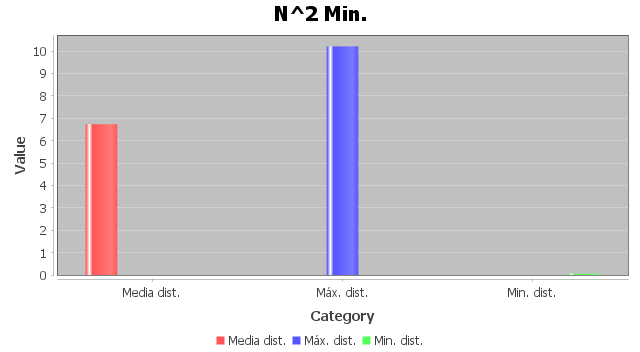
\includegraphics[width=\linewidth]{MVC/Controller/img/study_mean_distance.png}
    \caption{Estudio sobre la distancia media de una distribución uniforme}
    \label{fig:study}
\end{figure}

La razón por la que se limita el número de puntos verificados es para reducir el tiempo de ejecución del algoritmo. Al limitar el número de puntos verificados, podemos reducir el tiempo de ejecución del algoritmo y aun así encontrar el par (o pares) de puntos más cercanos en la matriz de la franja con una precisión razonable.\\

Por ende, se modifica el caso base para que, una vez la franja de la sección es menor a siete, se lance un algoritmo de coste asintótico $O(n^2)$ para encontrar más rápidamente la solución.
